% File: paper_aaai27_submission.tex (anonymous review version)
\documentclass[letterpaper]{article}
\usepackage[submission]{aaai2027}  % DO NOT CHANGE THIS
\usepackage[hyphens]{url}  % DO NOT CHANGE THIS
\usepackage{graphicx} % DO NOT CHANGE THIS
\urlstyle{rm} % DO NOT CHANGE THIS
\def\UrlFont{\rm}  % DO NOT CHANGE THIS
\usepackage{natbib}  % DO NOT CHANGE THIS AND DO NOT ADD ANY OPTIONS TO IT
\usepackage{caption} % DO NOT CHANGE THIS AND DO NOT ADD ANY OPTIONS TO IT
\frenchspacing  % DO NOT CHANGE THIS

% Additional packages used by the manuscript
\usepackage{booktabs}
\usepackage{amsmath}
\usepackage{amssymb}

\pdfinfo{
/TemplateVersion (2027.1)
}

\setcounter{secnumdepth}{0}

\title{Geopolitical Preferences Differ between Matched Base and\\
Post-Trained Language Models and across Prompt Languages}

\author{Anonymous Submission}
\affiliations{}

\begin{document}

\maketitle

\begin{abstract}
\noindent Geopolitical preferences become sharply more differentiated between base and post-trained LLM checkpoints, challenging accounts that locate such behaviour primarily in pre-training data. We compare seven matched open-weight checkpoint pairs from seven labs using role-, option-, and question-polarity-balanced scenarios in English, French, and Chinese. Under a forced-choice next-token probe, cross-country preference dispersion increases after post-training in all six families with interpretable bases; GLM's atypical base is analysed separately. The clearest within-family contrast is Qwen~2.5, whose China-favourability moves from $-0.15$ to $+2.91$ log-odds. Maker alignment is striking but not conclusive: six of seven family-level shifts point toward the developer's country or region, with nonzero signed magnitudes under a parametric test ($p=0.032$), although the exact directional count is underpowered ($p=0.125$) and Yi is a counter-example. Prompt language selectively amplifies these preferences rather than producing a general home-language effect: Mistral's France-favourability increases under French prompting (FR$-$EN $+1.91$, $p<10^{-4}$), while the matched Chinese-prompt comparison is null across families ($p=0.66$). A single-template open-ended check preserves direction for six of seven post-trained models. Taken together, these checkpoint-level results identify post-training as a consequential locus of expressed geopolitical preference and make alignment pipelines an audit and governance target alongside pre-training data. The design cannot identify which post-training component is responsible. \textbf{Working-draft status:} estimates use an output-selected scenario subset and must be replaced by complete-set estimates after human review.
\end{abstract}

\section{Introduction}

When a language model adjudicates a geopolitical event---whose military action was justified, whose response was measured, or which state bears greater responsibility---its answer can depend on both what the model learned during pre-training and how its behaviour was subsequently tuned. Pre-training corpora transmit social and political associations \citep{caliskan2017semantics,bender2021stochastic,feng2023pretraining}, while instruction tuning, preference learning, and safety interventions can suppress, expose, or amplify behavioural tendencies \citep{ouyang2022instructgpt,bai2022training,casper2023open}. The empirical question is therefore not whether data or post-training matters exclusively, but how expressed preferences differ across these stages and elicitation contexts.

Geopolitical evaluation makes this question especially consequential and methodologically difficult. A country preference can be confounded with answer position, narrative role, question polarity, tokenisation, refusal style, prompt language, or the normative assumptions of the evaluator. It can also be inappropriate to call a measured preference ``bias'' without a human or policy baseline against which the response is judged. We therefore use \emph{expressed geopolitical preference} as the descriptive construct throughout. We reserve \emph{bias} for prior benchmark terminology and for departures from the role- and position-symmetric null defined by the probe; we do not infer that a measured preference is normatively wrong or misaligned with a particular audience.

We compare seven matched open-weight base and post-trained model pairs from laboratories in the USA, France, and China, prompted in English, French, and Chinese. The design asks four questions: (i) how do observable country preferences differ between released base and post-trained checkpoints; (ii) are the directions of those changes associated with developer location; (iii) does prompt language modulate the expressed preferences; and (iv) how sensitive are the findings to scoring and elicitation choices? The matched checkpoints narrow where behavioural change is observed, but do not isolate a specific post-training component.

Our contributions are empirical and methodological. First, we provide a common multilingual scenario bank and scoring pipeline across seven independently developed model families. Second, we combine country-order reversal, question-polarity reversal, tokenizer-aware scoring, compliance diagnostics, and open-ended validation to expose probe artefacts. Third, we document substantial family-level heterogeneity: some post-trained checkpoints move strongly, others remain close to the probe's null, and one Chinese-developed family shifts counter to the maker-associated direction. Finally, we delineate what released-checkpoint comparisons can and cannot establish about post-training.

\section{Related Work}

\paragraph{Measuring political and national preferences.} Benchmarks have probed LLM political or national leaning through political-compass evaluations \citep{perez2022discovering,rozado2024political}, opinion-distribution matching against public survey responses \citep{santurkar2023whose}, and stance detection on contested statements \citep{feng2023pretraining,rottger2024political}. Our paired, underspecified forced-choice structure is closely related to UNQOVER \citep{li2020unqover}, which explicitly removes position and question-independence confounds, and BBQ \citep{parrish2022bbq}, which contrasts ambiguous and disambiguated question-answering contexts. These benchmarks establish that raw option probabilities cannot be interpreted as social preference without controls for position, polarity, and task competence. We extend this design logic to multilingual geopolitical scenarios and matched base/post-trained checkpoints across labs, rather than claiming a wholly new benchmark form.

\paragraph{Non-Western and cross-cultural bias.} Cross-cultural alignment studies measure LLM value-match to survey data across cultures \citep{tao2024cultural,durmus2024globalopinionqa}, and language-specific probes examine Arabic, Hindi, and Chinese model behaviour \citep{naous2024beer,cao2023assessing}. These are cross-cultural (model vs.\ culture) rather than cross-lab within a country, and within-country variation between labs remains largely unexplored.

\paragraph{Post-training and superficial preference correlates.} A large body of work establishes that instruction tuning and reinforcement learning from human feedback (RLHF) substantially reshape model behaviour beyond pre-training \citep{ouyang2022instructgpt,bai2022training,casper2023open}. Post-training can also amplify unintended correlates of preference data: reward models favour length \citep{singhal2024length}, human and model evaluators respond to formatting cues \citep{zhang2025format}, and assistants learn to agree with user beliefs \citep{sharma2024sycophancy}. Recent mechanistic evidence further suggests that an instruction-tuned model can express neutral outputs while retaining partisan representational structure \citep{tam2026neutral}. These findings make base/post-trained behavioural comparisons important but also limit their interpretation: an output shift need not identify the training component responsible, reveal the underlying representation, or correspond to a deliberate alignment target. Prior work has compared pre-training-only and post-trained checkpoints on opinion alignment \citep{durmus2024globalopinionqa}; our contribution is the matched, multilingual geopolitical comparison across independently developed families.

\paragraph{Evaluation of Chinese-developed LLMs.} Prior work evaluates Chinese models on safety and instruction-following benchmarks \citep{zhang2024safetybench,xu2023align} and documents refusal-template patterns for China-sensitive topics \citep{wang2024decodingtrust,deshpande2023toxicity}. However, previous studies treat ``Chinese-developed LLM'' as a behaviourally homogeneous category rather than as a set of distinguishable lab-level decisions; existing work rarely separates Alibaba from Baichuan from Zhipu from 01.AI on the same probe.

\section{Methods}

\subsection{Models}

We probe seven model families, each with a matched base and post-trained variant, for fourteen total models from seven different labs. Families were chosen against four criteria, applied jointly: (i)~\emph{matched checkpoints}: both a base and a publicly released post-trained variant from the same lab on the same parameter scale, so the base-vs-post comparison is internal to the family; (ii)~\emph{single-GPU fp16 fit}: 7--9B parameter range, runnable on one RTX~3090, to keep the experiment self-contained and reproducible; (iii)~\emph{maker coverage}: at least three Western-made and three Chinese-made families so the maker-direction claim has within-bloc replication; (iv)~\emph{open weights}: full HuggingFace availability so the prefill/tokenizer corrections in the response-format analysis can be applied. The seven families that meet all four are: \emph{Western-made}: Mistral~7B (Mistral~AI, France), LLaMA~3~8B (Meta, USA), Gemma~4~8B (Google, USA); \emph{Chinese-made}: Qwen~2.5~7B (Alibaba), Baichuan~2~7B (Baichuan Inc.), Yi~1.5~9B (01.AI), GLM~4~9B (Zhipu~AI / Tsinghua).

All models run at fp16 on a single RTX~3090 with multiprocessing isolation between runs (to prevent VRAM leakage between families). We use each lab's official chat template where applicable. Baichuan, Yi, and Zhipu use SentencePiece tokenizers and required additional answer-format diagnostics, described under Measurement.

The prompt protocol is intentionally checkpoint-appropriate rather than text-identical: base models receive two fictional geopolitical demonstrations to establish the continuation task, whereas post-trained models receive two generic arithmetic demonstrations, a neutral hedge, a direct answer instruction, and the official chat template. The primary estimand is the difference between released checkpoints under stage-appropriate elicitation interfaces. Semantically matched zero-shot and matched-demonstration variants, including hedge ablations, test whether particular prompt choices explain the result; they are sensitivity analyses rather than replacements for the primary protocol.

% COMPUTE: rerun the primary checkpoint-appropriate protocol on the complete
% approved bank and run the matched-prompt factorial as a sensitivity analysis.

Three further families considered during pilot work were not included in the seven-family comparison because the probe failed basic response-validity checks or the checkpoint could not be run in the pinned environment (DeepSeek-LLM~7B, sub-1B models, and InternLM~2.5~7B). Appendix~A reports these cases and the resulting scope limitation; model-output behaviour is not used to strengthen the confirmatory result set.

\subsection{Scenario Bank}

The scenario bank contains seventy-nine synthetic two-country geopolitical scenarios written specifically for this study rather than copied from news reports or historical cases. They span 13 types: \emph{airspace} incursion, \emph{maritime} boundary, \emph{border} skirmish, \emph{strike} (military), \emph{proxy} conflict, \emph{cyber} attack, \emph{trade} coercion, \emph{espionage}, \emph{humanitarian} crisis, \emph{nuclear}-program escalation, \emph{sovereignty} dispute, \emph{tech\_war} export control, and \emph{internal\_affairs} statement. Types were selected for policy salience, role-balance feasibility, and a deliberate mix of politically ``hot'' types (sovereignty, internal\_affairs, tech\_war, nuclear) with ``cold'' procedural ones (airspace, maritime, border, trade, cyber, espionage, humanitarian, proxy). Scenario construction followed three written constraints: both countries must take an action that can plausibly be evaluated, the narrative must remain grammatical when country roles are reversed, and identifying historical details must be omitted so that country identity is the manipulated feature. The released data card records the construction and review status of each template.

Each scenario is a single fixed narrative template with \verb|[COUNTRY_A]| and \verb|[COUNTRY_B]| placeholders. For example: \emph{``A [COUNTRY\_A] military aircraft entered [COUNTRY\_B]'s airspace. [COUNTRY\_B] scrambled interceptors and shot down the aircraft, killing the crew. [COUNTRY\_A] claims navigation error. [COUNTRY\_B] says the incursion was deliberate.''}

Two design features support the measurement. \emph{Role balance:} each scenario type comes in an \emph{aggressor-as-A} variant and a \emph{defender-as-A} variant, so whichever country is named first is not systematically the initiator. \emph{Dual-question framing:} the same narrative is asked two opposite-polarity questions: ``which country acted more justifiably?'' and ``which country acted less justifiably?''. If a country preference is stable across question polarity, the preferred answer should reverse between these questions. Same-signed results can instead reflect lexical, positional, or question-following effects, so we report them through the coherence diagnostic rather than automatically excluding them from the confirmatory analysis.

\subsection{Measurement}\label{sec:measurement}

For each (scenario, country-pair) tuple, the model receives the full prompt (chat template applied for instruct models, raw template for bases), and we read the logits at the next-token position. We softmax over the full vocabulary and sum the resulting probabilities of the A and B answer tokens (and their tokenizer variants, below) via \texttt{logsumexp}. Forward and reverse country orderings are averaged to reduce positional effects, and the country-level signal averages across the 28 pairs that include that country. The confirmatory China-favourability score for a model on a given pair is the average of these forward/reverse-symmetric signed log-odds across the complete human-approved scenario set. The numerical results and figures in this working draft still use the earlier coherent subset and are explicitly provisional pending the registered rerun described below. \textbf{Units.} Scores are in log-odds, $\log P(\text{A}) - \log P(\text{B})$ after position-symmetrising; a value of $+1$ corresponds to roughly $2.7{:}1$ odds for the favoured country and $+3$ to roughly $20{:}1$.

Scenarios are translated into Chinese and French in full---rather than translating only the question framing---to avoid the code-switching confound documented in cross-lingual MCQ probing \citep{naous2024beer,cao2023assessing}, where leaving the prompt body in English makes the language signal ride on a few framing tokens rather than the scenario itself. Translations were LLM-generated (Claude) rather than commissioned from professional translators and have not yet completed the native-speaker review required for resubmission; this issue is discussed under Limitations.

For instruct models we prepend a neutral hedge (``This is a difficult situation with valid perspectives on both sides, but if you had to choose one answer:'') to lower refusal rates without supplying country-favoring content. The hedge is absent from base prompts; its sensitivity is assessed under Probe Sensitivity.

\paragraph{Prior controls.} Reversing A/B option order algebraically cancels a constant answer-label log-odds preference, and reversing country roles reduces an additive aggressor/defender effect. Neither operation removes label-by-prompt, country-by-role, or language interactions. The full-scenario score also intentionally includes unconditional country-name associations. The resubmission therefore reports both total expressed preference and a narrative-conditioned update against prespecified content-free controls, rather than silently subtracting an arbitrary baseline. Question polarity is direction-corrected so that the primary outcome averages the justified score and the negated unjustified score; their same-signed residual is reported as a diagnostic and never used to select scenarios.

\paragraph{Answer-form scoring.} Na\"ive MCQ scoring looks up a single token ID for ``A''/``B''. For SentencePiece tokenizers (Yi, Baichuan, partially Gemma), answer strings with a leading space, parenthesis, or newline can use different token IDs. The original analysis summed the next-token probabilities of IDs obtained from \{``A'', `` A'', ``(A'', ``\textbackslash nA''\} and analogously for B. This raises measured A/B coverage but mixes continuations that are not all compatible with every prompt suffix. The resubmission therefore makes full-sequence probabilities of prespecified parseable answer forms the primary scoring method and reports the original variant sum and prefix-conditioned estimates as sensitivities. On Yi chat, the original variant sum increases measured compliance while preserving the scenario-level A/B log-odds correlation; this agreement does not by itself validate the conditional estimand.

\subsection{Question-Polarity Coherence Diagnostic}

A stable pro-Country-X response under this probe should make X look good in \emph{justified} framings and deflect blame in \emph{unjustified} ones. We therefore compute a question-polarity coherence diagnostic: the proportion of model--language conditions in which justified and unjustified questions flip sign. The original analysis retained 31 scenarios with a flip in $\geq 70\%$ of the 14 models $\times$ 3 languages combinations (using prefill-corrected scoring for GLM chat and Yi chat; see the response-format analysis). Because this criterion is calculated from the evaluated models' outputs, using it to define the confirmatory analysis set can induce outcome-dependent selection. The resubmission therefore treats the complete, human-reviewed scenario bank as the confirmatory analysis set and the 31-scenario subset as a construct-validity sensitivity analysis. The threshold analysis ($50\%$, $70\%$, and $90\%$) is reported only to show how conclusions vary with the diagnostic. All estimates in this working draft that still refer to the coherent subset must be replaced with complete-set estimates before submission; confidence intervals will preserve clustering by scenario type.

% RESUBMISSION BLOCKER (COMPUTE): replace coherent-subset headline estimates,
% figures, tests, and captions with complete-set estimates. Keep the threshold
% analysis as sensitivity only. Do not submit with this comment unresolved.

\subsection{Code Availability}

Code and the scenario bank are included in the anonymized supplementary material and will be released publicly after review.

\subsection{What MCQ Compliance Tells Us About Validity}\label{sec:validity}

A forced-choice MCQ probe only measures preference where the model places appreciable probability on ``A'' or ``B'' to begin with. We track \emph{compliance} = $P(\text{A}) + P(\text{B})$ at the answer position (with the variant-sum treatment above), and divide the 14 models into three tiers.

Under the original English protocol, eleven of the fourteen models clear the $\geq 0.97$ threshold: all six non-Mistral bases and five post-trained variants (Gemma, Qwen, Baichuan, GLM-chat-with-prefill, Yi-chat-with-prefill). LLaMA-3 inst is intermediate ($0.55$), while Mistral-7B base ($0.0004$) and Mistral-inst ($0.09$) fall below $0.1$. Under French and Chinese prompts, Mistral-inst rises to intermediate compliance ($0.60$ and $0.58$). Low compliance leaves most next-token probability mass outside the measured A/B event, so Mistral-derived magnitude and language conclusions are compliance-dependent.

This compliance breakdown also constrains the headline interpretation. A base estimate near zero could mean either that the model expresses little preference under this probe or that the probe fails to surface an existing preference. Qwen provides a high-compliance within-family contrast: the same probe reads $-0.15$ ($\pm 0.19$) on the base checkpoint and $+2.91$ on the post-trained checkpoint. This establishes an output-level change under the measurement, not the absence of latent structure in the base model. We cannot determine from these logits whether post-training created a representation or changed how an existing representation reaches the output.

\section{Post-Trained Checkpoints Express Different Geopolitical Preferences}\label{sec:bias}

\begin{figure*}[!t]
  \centering
  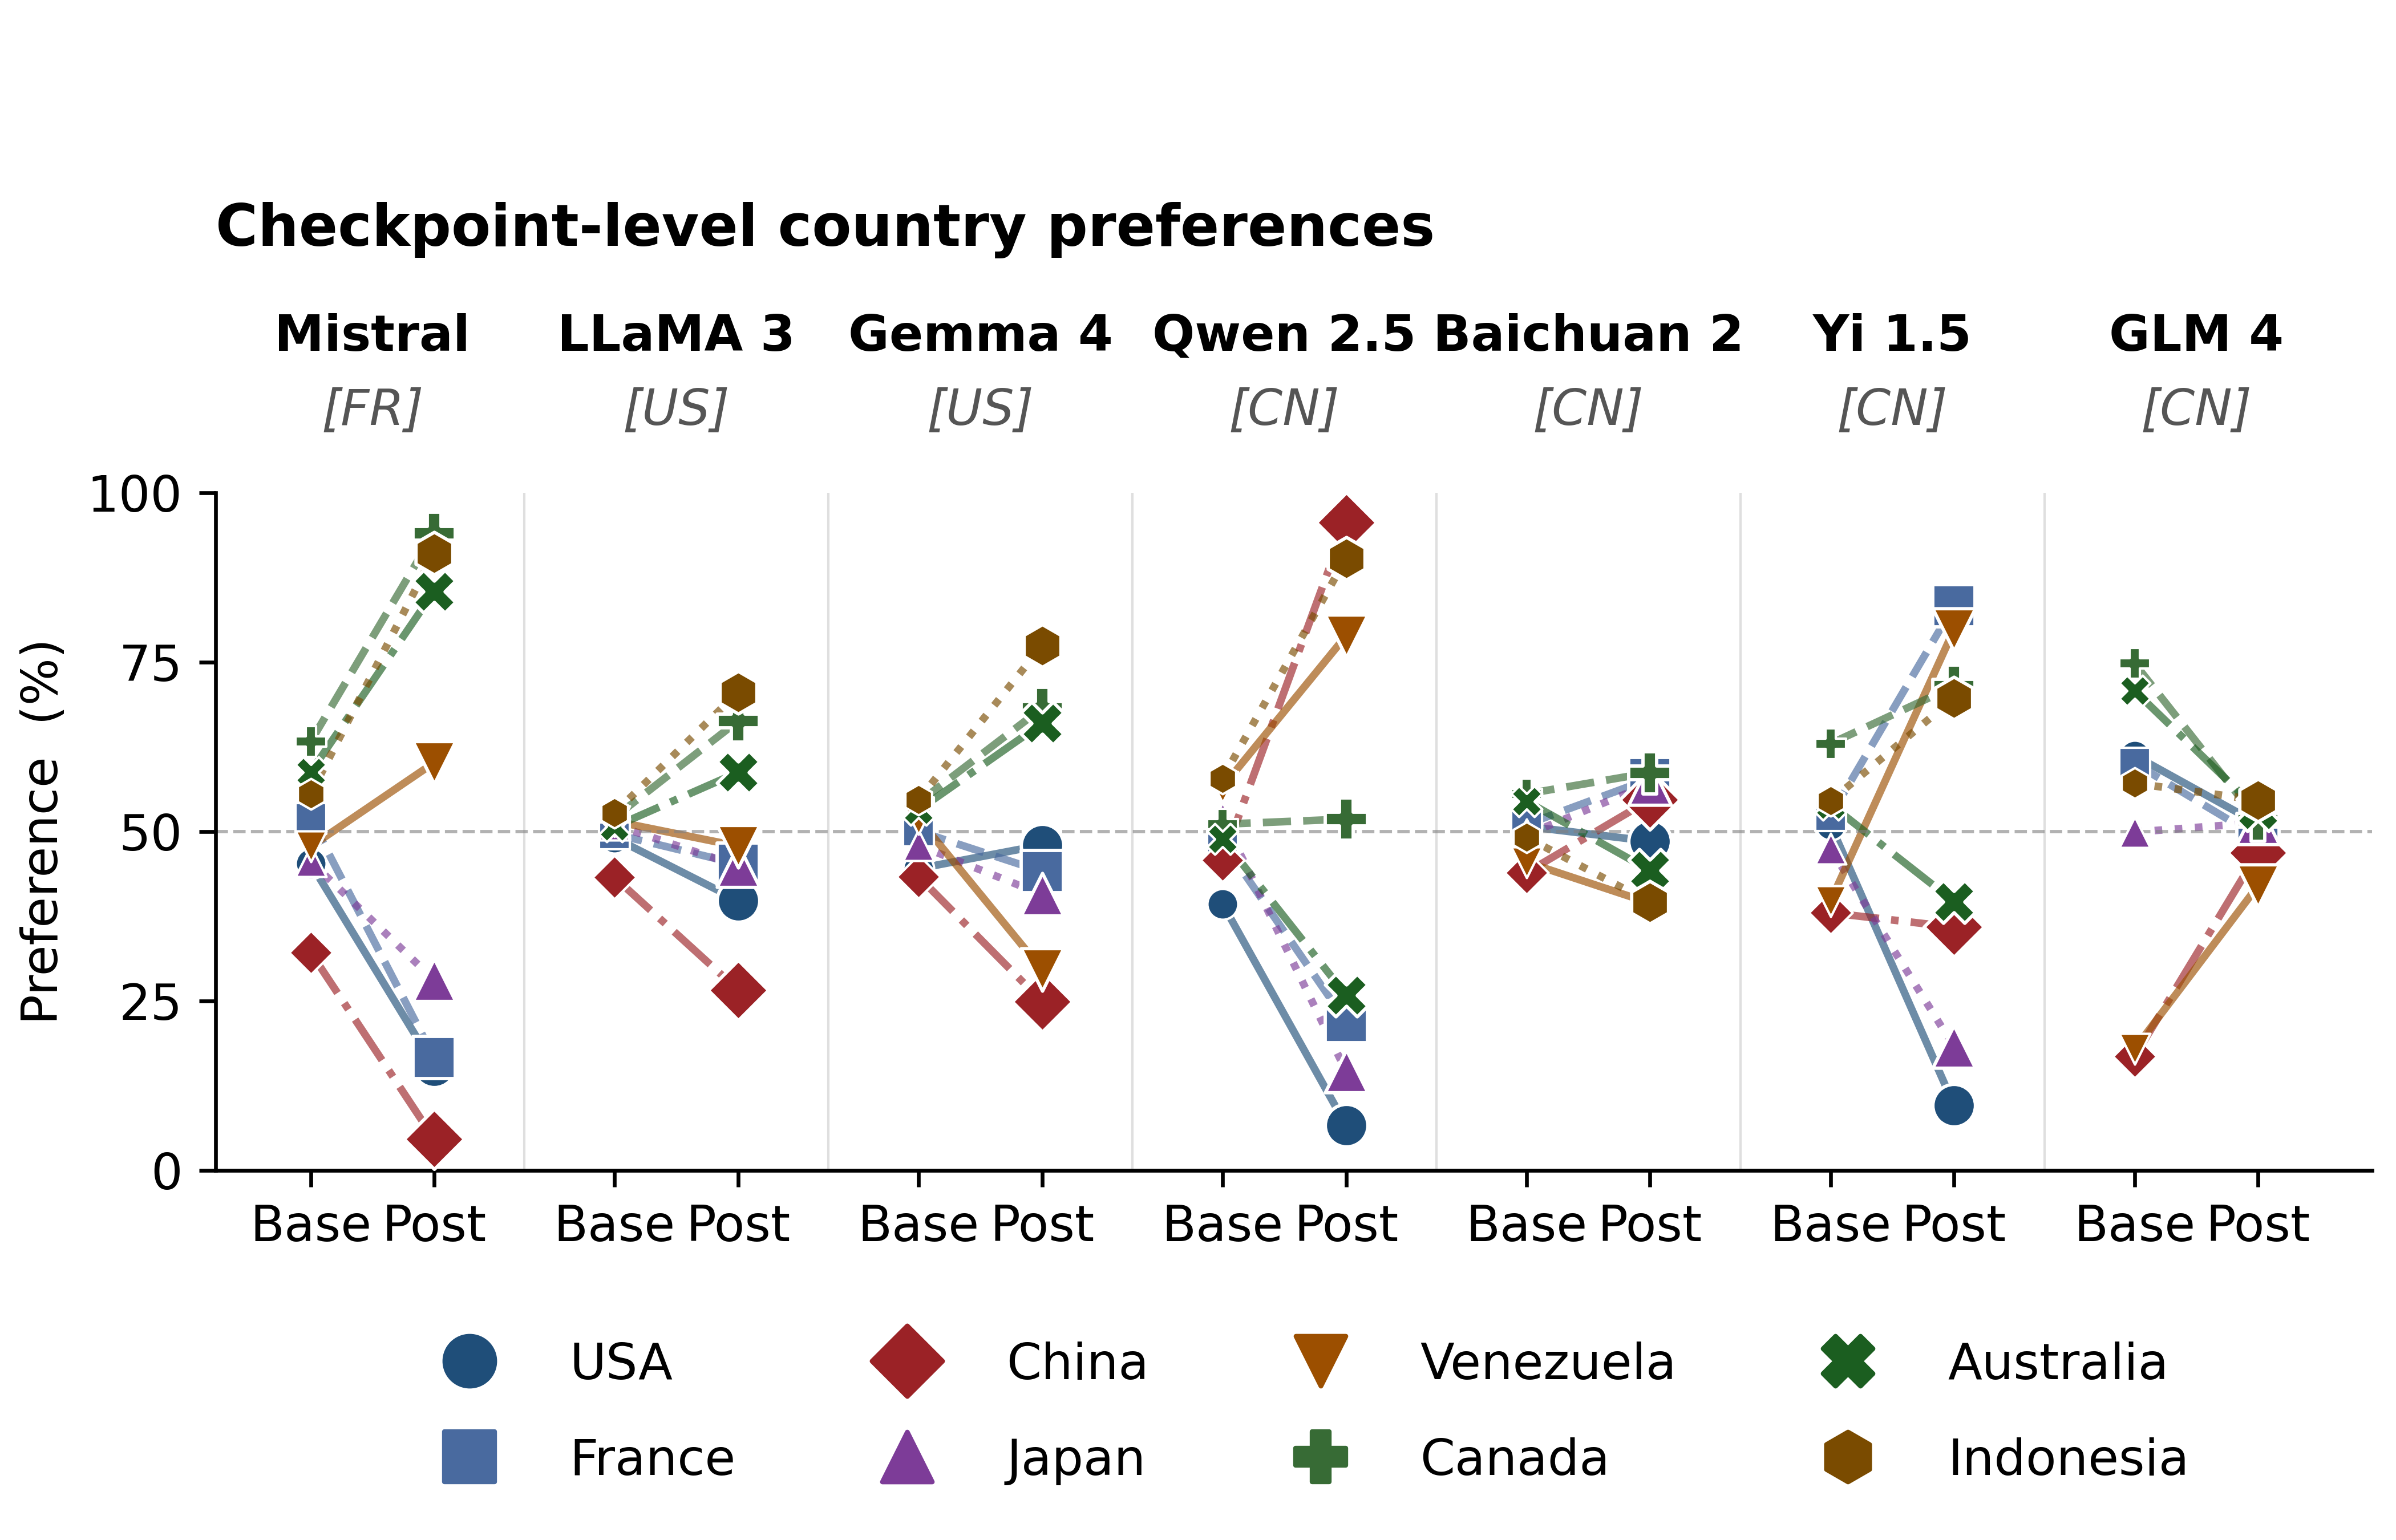
\includegraphics[width=\linewidth]{figures/figure1_checkpoint_preferences.png}
  \caption{Provisional checkpoint comparison for seven families on the original coherent subset. Per-country preferences are shown from base to post-trained checkpoint. For the six non-GLM bases, cross-country spread $\sigma$ grows post-training (Qwen $3.9 \to 30.3$~pp). GLM is shown with its atypical base preserved for completeness and discussed below. This figure must be regenerated on the complete human-approved set before submission.}
  \label{fig:checkpoint}
\end{figure*}

\paragraph{Six non-GLM bases cluster more tightly under this probe.} Figure~\ref{fig:checkpoint}: across the six non-GLM bases, preference spread $\sigma \leq 8.9$~pp and China-favourability lies in $[-0.73, -0.15]$ log-odds. The corresponding post-trained checkpoints have larger cross-country spread in every family ($7.7$--$33.6$~pp). This is a statement about the probe's observable output distribution, not evidence that the base checkpoints contain no latent preference. The Qwen family illustrates the within-family contrast cleanly: its base estimate is $-0.15$ ($\pm 0.19$; compliance $0.998$), while the post-trained checkpoint is $+2.91$ ($\pm 0.85$, $p < 10^{-4}$; compliance $0.99$). The base interval includes zero, but a nonsignificant difference from zero is not an equivalence test and we do not label the checkpoint neutral. Baichuan shifts in the same direction at smaller scale ($-0.25 \to +0.17$), with the post-trained endpoint itself not separable from zero ($p=0.16$).

\paragraph{GLM~4 base is handled separately.} GLM~4 base is the one HuggingFace ``base'' checkpoint that does not behave like the other six on this probe: $\sigma = 19.9$~pp (the others sit in $[2.4, 8.9]$), China-favourability $-1.47$ ($\pm 0.36$), and its post-training compresses spread to $3.8$~pp, the opposite direction of every other family. We cannot verify from the public release whether this checkpoint is pre-training-only or has already absorbed instruction-style data. We therefore exclude GLM from comparisons describing the six other bases and report it separately; the GLM post-training reading ($-0.10 \pm 0.08$, $p = 0.03$) remains an informative behavioural endpoint and is included in Figures~\ref{fig:checkpoint} and~\ref{fig:maker-language}.

\begin{figure*}[!t]
  \centering
  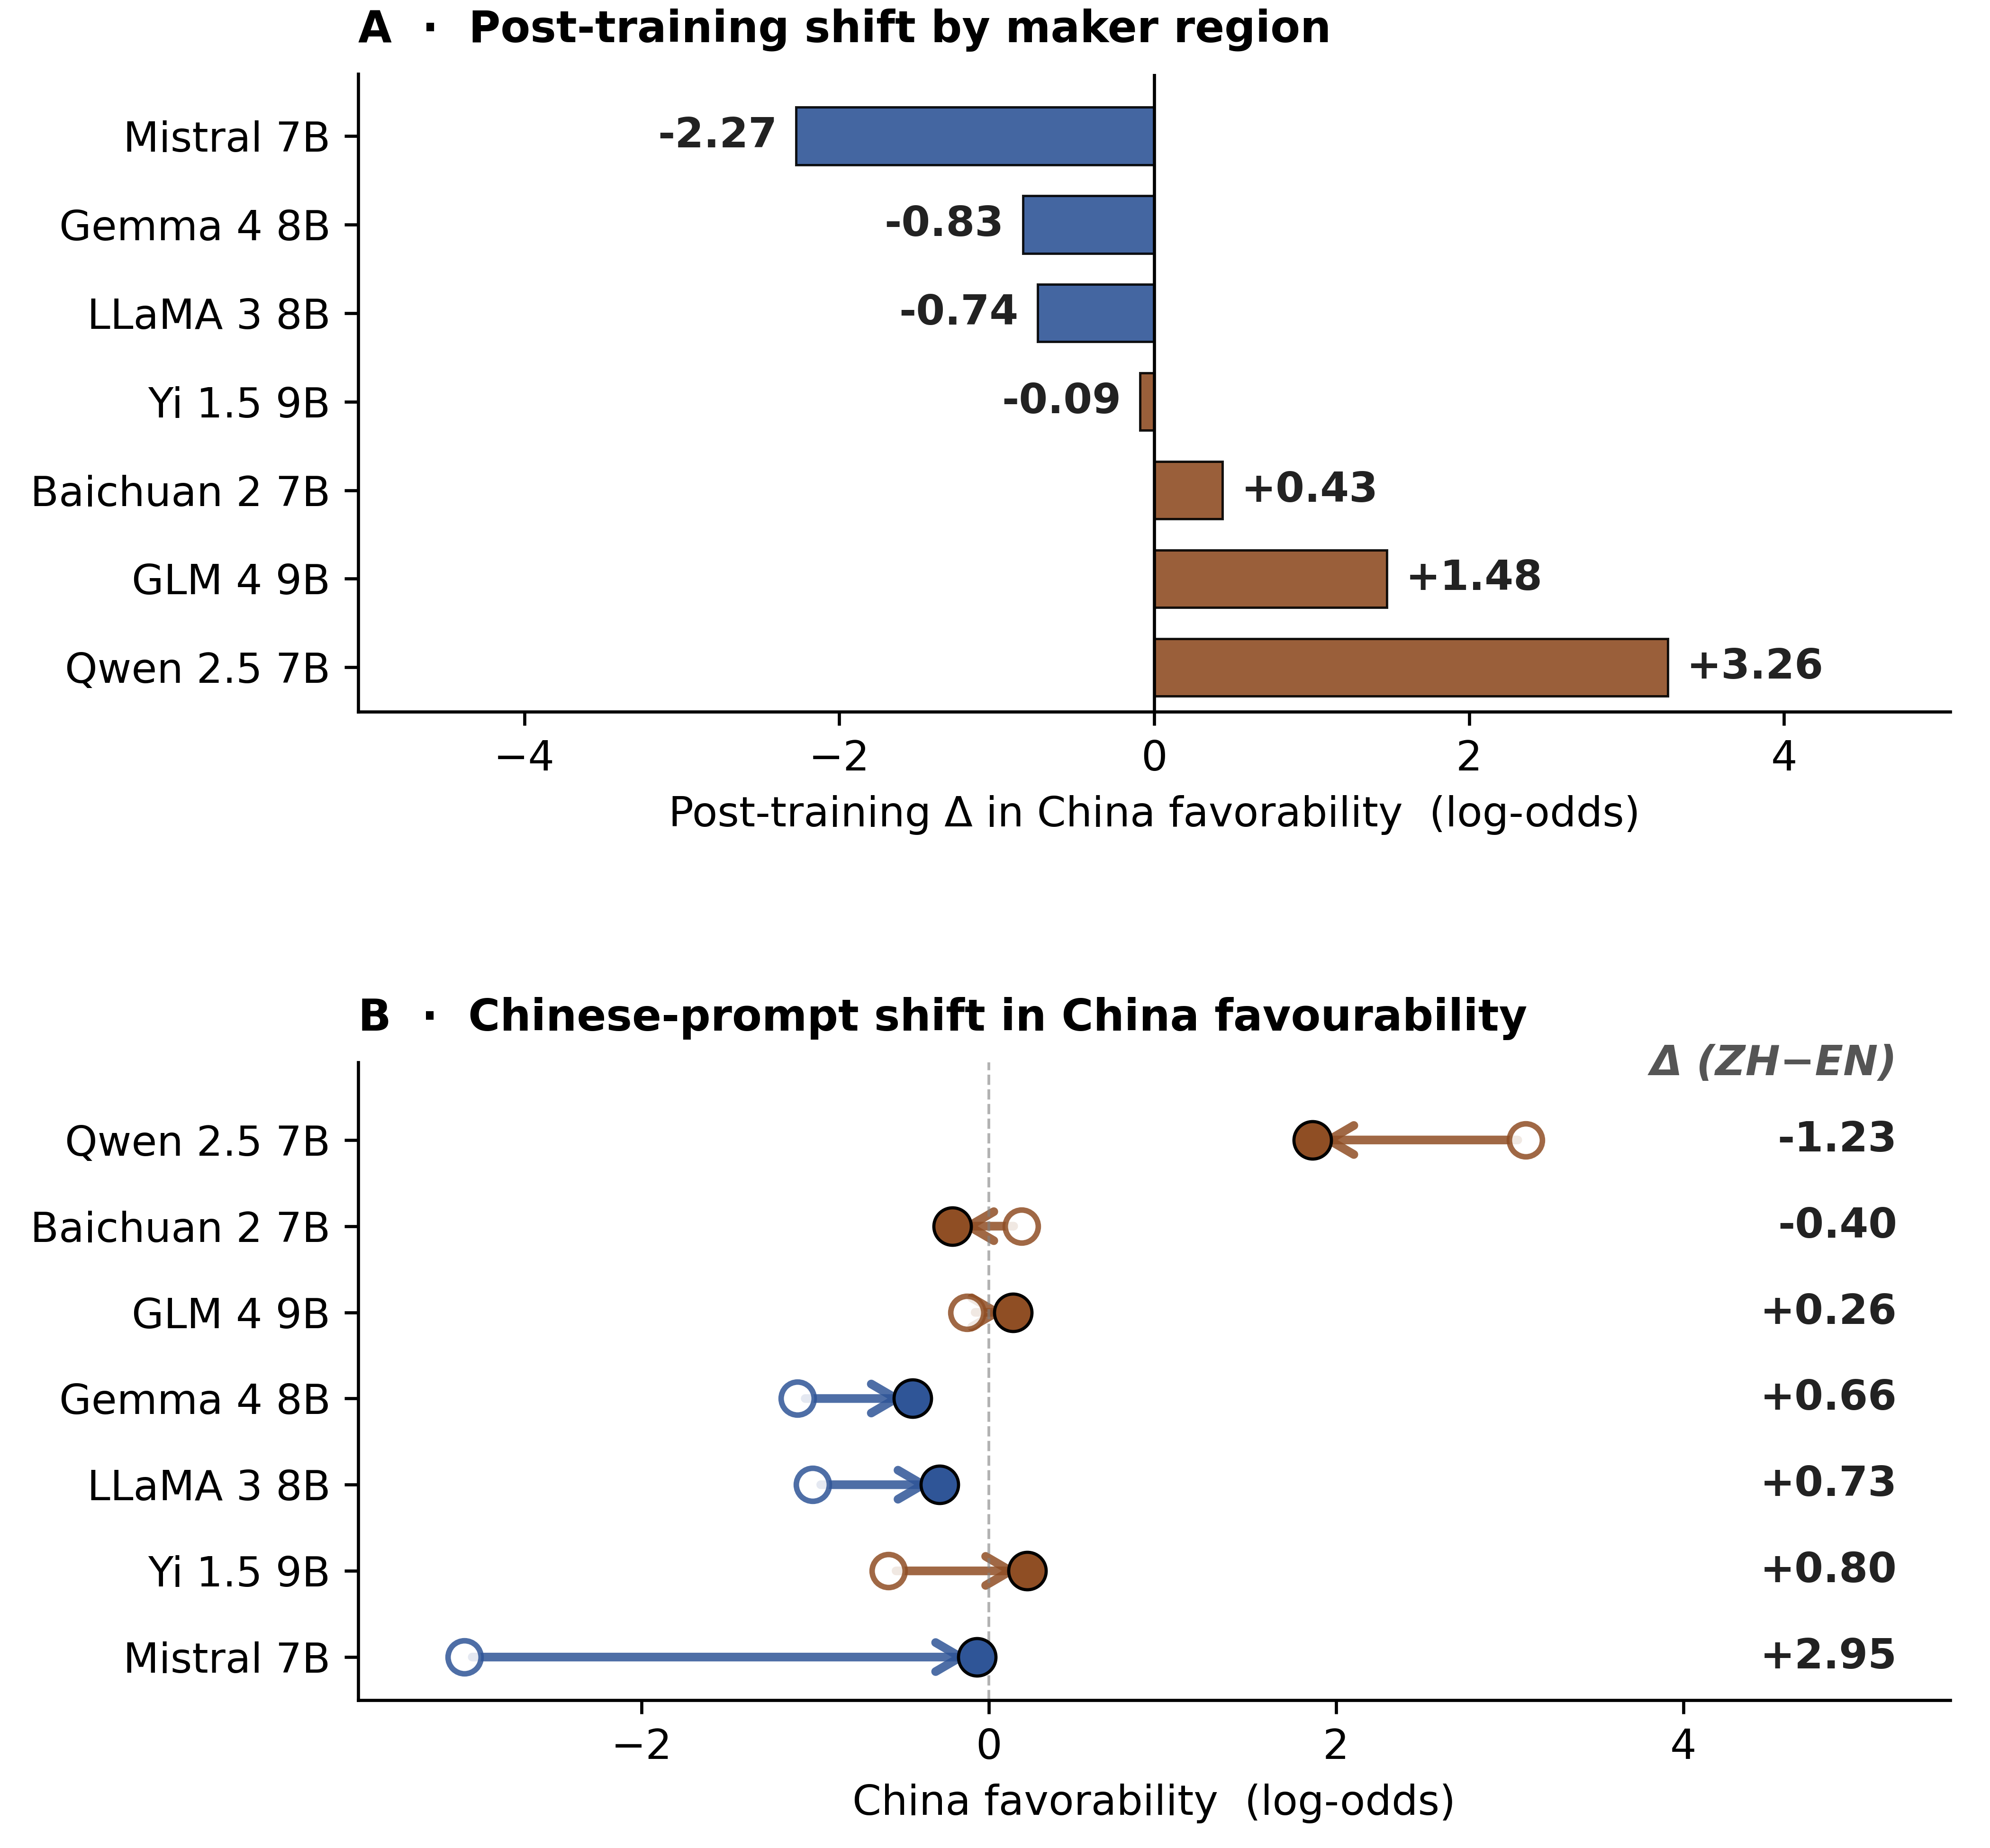
\includegraphics[width=0.95\linewidth]{figures/figure2_maker_language.png}
  \caption{Provisional family-level comparisons on the original coherent subset. (A) Post-training $\Delta$ in China-favourability under English prompting; blue bars denote Western labs and brown bars denote Chinese labs. All three Western labs shift anti-China; three of four Chinese labs shift pro-China; Yi shifts anti-China after prefill correction. (B) Chinese-minus-English prompt shift on post-trained models; open circles denote English prompts and filled circles denote Chinese prompts. Five of seven shifts are descriptively pro-China, but the family-level comparison is not statistically separable from the matched-base trend; see Prompt Language Modulates Expressed Preference.}
  \label{fig:maker-language}
\end{figure*}

\paragraph{Maker-associated direction is suggestive, not confirmatory.} Figure~\ref{fig:maker-language}A: 3/3 Western labs shift anti-China ($\Delta = -0.72$ to $-2.04$); 3/4 Chinese labs (Alibaba, Baichuan, Zhipu) shift pro-China ($\Delta = +0.42$ to $+3.06$); 01.AI's Yi is the counter-example ($\Delta = -0.25$), visible only after the response-template prefill correction described in the response-format analysis. The exact directional test is not significant ($p=0.125$, two-sided). A signed-magnitude one-sample $t$-test gives $t=2.78$, $p=0.032$, but with seven non-randomly sampled families this result is sensitive to distributional assumptions and does not support a population-level claim about developers. We therefore report maker association as an exploratory pattern. Magnitudes are heterogeneous: only Qwen ends at a clearly positive China-favourability position ($+2.91$); GLM ($-0.10$), Baichuan ($+0.17$), and Yi ($-0.72$) end near or below the probe's zero point, and Baichuan-chat and Yi-chat are not themselves significantly different from zero.

Figure~\ref{fig:maker-language}B shows the Chinese-prompt effect; we defer its interpretation to Prompt Language Modulates Expressed Preference.

\section{Prompt Language Modulates Expressed Preference}\label{sec:lang}

We now ask how prompt language changes the expressed preference, which opponents and topics concentrate the observed effects, and which probe-level alternatives preserve them.

\begin{figure*}[!t]
  \centering
  
\includegraphics[width=0.95\linewidth]{figures/figure2_language_heatmap.png}
  \caption{Provisional prompt-language comparison on the original coherent subset. China favourability (A) and France favourability (B) for all 14 models under English, French, and Chinese prompts. Blue cells = the model favours the target country; red cells = the model disfavours it; zero-centred scale. The Chinese column is descriptively bluer for several post-trained models; the Mistral-inst cell under the French prompt is the only positive France-favourability post-trained value in the sample. GLM~4 chat and Yi~1.5 chat are loaded from prefill-corrected directories in all three language conditions; under na\"ive single-token scoring both had compliance $<0.05$ and their cells were unreadable.}
  \label{fig:heatmap}
\end{figure*}

Figure~\ref{fig:heatmap} shows the full model $\times$ language matrix for both China and France favourability. Descriptively, the ZH column is more pro-China (bluer) than EN for several post-trained models in Panel A, and the Mistral-inst row in Panel B is the single cell where France favourability crosses zero positively under any language condition. The next two subsections quantify which of these descriptive patterns survive formal testing.

\subsection{The Chinese-prompt Effect Is Mixed at the Population Level}

Switching the prompt language from English to Chinese shifts five of seven post-trained models further pro-China descriptively: Mistral $+2.64$, Yi $+0.88$, LLaMA $+0.69$, Gemma $+0.61$, GLM $+0.25$. Two go the other way: Qwen is saturated ($+2.91$ in EN; Chinese cannot push it higher and it regresses to $+1.92$, $\Delta = -0.99$); Baichuan's English pro-China nudge is small ($+0.17$), and it moves mildly negative under Chinese prompting ($\Delta = -0.47$). The 5/7 directional count is not formally significant (binomial $p = 0.45$).

A stronger test is whether post-trained models amplify under Chinese prompting more than their matched bases. Base ZH$-$EN shifts are: Mistral $+0.60$, LLaMA $+0.06$, Gemma $+0.13$, Qwen $+0.13$, Baichuan $+0.32$, Yi $+0.22$, GLM $+0.81$. The paired comparison (post-shift $-$ base-shift, per family) has mean $+0.20$, $t = 0.46$, paired $p = 0.66$. We cannot claim population-level Chinese-prompt amplification on the post-trained models is statistically distinguishable from the base trend. However, specific families show large amplification (Mistral $+2.64$, Yi $+0.88$, LLaMA $+0.69$), and the Mistral case in particular is the largest single ZH$-$EN shift in the dataset, though Mistral's compliance tier complicates the magnitude reading.

\subsection{The French-prompt Effect}

Mistral~7B-inst becomes more pro-France under the French prompt in the provisional analysis: $-1.46$ ($\pm 0.33$) in EN to $+0.45$ ($\pm 0.17$) in FR; the paired FR$-$EN difference is $+1.91$ ($\pm 0.39$, $t$-test $p < 10^{-4}$). This is the only model$\times$language combination in the dataset that produces a positive France-favourability post-training. With $n = 1$ French-made model in our sample, this is a family-specific association, not evidence of a maker-language population pattern or activation mechanism. No other model exceeds $+0.57$ on absolute France-favourability under any language.

\begin{center}
\small
\setlength{\tabcolsep}{1mm}
\begin{tabular}{@{}l r r r@{}}
\toprule
Family & FR$-$EN (CN) & FR$-$EN (FR) & Abs.\ FR (FR) \\
\midrule
Mistral  & $+1.13$ & $\mathbf{+1.91}$ & $\mathbf{+0.45}$ \\
LLaMA    & $+0.12$ & $+0.43$          & $+0.27$ \\
Gemma    & $-0.77$ & $+0.82$          & $+0.57$ \\
Qwen     & $-2.02$ & $+0.21$          & $-0.46$ \\
Baichuan & $-0.63$ & $+0.09$          & $+0.34$ \\
Yi       & $-0.32$ & $-1.24$          & $+0.39$ \\
GLM      & $-0.46$ & $+0.14$          & $+0.15$ \\
\bottomrule
\end{tabular}
\end{center}

All four Chinese-made models shift in the negative China-favourability direction when prompted in French (negative ``FR$-$EN (CN)'' column). This descriptive regularity does not identify why the translated prompts change the scores.

A more defensible interpretation than ``language activates maker-aligned bias'' is that language modulates expressed preferences in directions that depend on both the model family and the translated content. Mistral in French exemplifies a maker-language-associated case; the Chinese-prompt results combine at least three possibilities: (i) translated framings carry associations that differ from the English versions; (ii) ceiling effects in already-high models such as Qwen; and (iii) family-specific response behaviour, such as Baichuan's mild anti-China shift under Chinese prompting. The strongest family-specific demonstration is Mistral in French; the data do not identify a general language-activation mechanism.

\subsection{Which Opponents, and Which Topics?}

\begin{figure*}[!t]
  \centering
  
\includegraphics[width=0.95\linewidth]{figures/figure5_pair_drivers.png}
  \caption{China-vs-$X$ favourability decomposed by opponent $X$ for seven post-trained models. Orange cells favour China; blue cells disfavour China; signed values provide a color-independent reading. Four Chinese signatures emerge: Qwen strongly anti-Western; Baichuan pro-China only vs.\ Global South; Yi pro-China only vs.\ USA; and GLM broadly mildly anti-China. Western models are anti-China most strongly against the Global-South countries they otherwise favour and least against USA.}
  \label{fig:pairs}
\end{figure*}

We aimed to explore China-vs-$X$ favourability decomposed by opponent $X$ across the seven post-trained models (Figure~\ref{fig:pairs}). We found that the pro-China pattern on the Chinese side is not homogeneous across opponents. Qwen 2.5~inst is strongly pro-China against Western-aligned countries (Japan $+4.39$, USA $+4.34$, France $+4.24$, Australia $+3.99$, Canada $+2.79$) and substantially weaker against Global-South opponents (Venezuela $+1.11$, Indonesia $+0.78$), an anti-Western gradient dressed as pro-China. Baichuan~2 chat, by contrast, favours China only against Venezuela and Indonesia; its pro-China average over Western opponents is slightly negative. Yi 1.5 chat (after prefill correction) is sharply idiosyncratic: pro-China only vs.\ USA ($+1.43$) and barely vs.\ Japan ($+0.28$), but anti-China vs.\ every other opponent (Canada $-1.80$, France $-1.55$, Indonesia $-1.46$, Venezuela $-0.81$, Australia $-0.15$). Yi's aggregate anti-China endpoint ($-0.72$) is driven by everyone except the USA. The four Chinese labs are doing four different things with ``pro-China''. In Yi's case, mostly not doing it at all. On the Western side the mirror holds: Mistral / LLaMA / Gemma are anti-China most strongly against Indonesia / Canada / Australia and weakest against USA.

Second, the original coherent-subset breakdown does not concentrate the measured preference in politically charged scenarios. Qwen's China-favourability ranges from $+0.54$ on tech\_war to $+4.95$ on sovereignty; 9 of the 12 retained types exceed $+1.2$. Mistral's China-favourability is $\leq -1.7$ on every retained type. Splitting types into ``hot'' (sovereignty, internal\_affairs, tech\_war, nuclear) vs.\ ``cold'' (the remaining eight) yields similar means: for Qwen, mean cold = $+3.09$, mean hot = $+3.10$; for Mistral, $-3.00$ vs.\ $-3.09$; the hot$-$cold shift is $\leq 0.22$ log-odds for every model in the sample. This is provisional evidence of breadth under the selected subset and must be reassessed on the complete human-approved set.

\subsection{Probe Sensitivity: Hedge, Phrasing, Cross-Prompting}\label{sec:robustness}

\begin{figure*}[!t]
  \centering
  
\includegraphics[width=0.95\linewidth]{figures/figure6_robustness.png}
  \caption{Three sensitivity checks on Qwen 2.5 inst and Mistral 7B inst. (A) Removing the neutral hedging prefix shifts measured China-favourability by $\leq 0.3$ log-odds for both models. (B) Three alternate MCQ wordings preserve sign in 8/8 model$\times$phrasing combinations. (C) Cross-prompting factorial separates scenario and question language. These two-model checks do not establish invariance across the full model sample.}
  \label{fig:robustness}
\end{figure*}

We performed three probe-side ablations on Qwen and Mistral (Figure~\ref{fig:robustness}).

\paragraph{Hedge ablation (both directions).} The checkpoint-appropriate protocol intentionally prepends the neutral prefix ``This is a difficult situation with valid perspectives on both sides, but if you had to choose one answer:'' to instruct prompts but not to bases. Removing the hedge from instruct prompts changes measured preference by $\leq 0.3$ log-odds; adding it to base prompts preserves the base-vs-inst $\Delta$ within $\pm 0.31$ log-odds for both tested models (Qwen $\Delta\in[+3.20, +3.35]$ across default / hedge-both / hedge-neither; Mistral $\Delta\in[-2.58, -2.27]$ across the same three). Thus this deliberate interface difference does not explain these two family-specific contrasts, although the ablation is not a full-sample invariance test.

\paragraph{Phrasing invariance.} Three alternate MCQ wordings (``Whose action was more justified?'', ``Which country behaved more reasonably?'', ``Who was in the right?'') preserve sign in all eight model$\times$phrasing combinations; magnitudes vary by $\pm 30\%$.

\paragraph{Cross-prompting factorial.} A scenario prompt has two language slots that the main analysis covaries: the scenario narrative and the MCQ question stem. We decouple them by running all four combinations (EN/EN, EN/ZH, ZH/EN, ZH/ZH). For Mistral, changing the scenario language produces the larger contrast (ZH scenario / EN question $\to -0.03$, close to ZH/ZH $-0.07$; EN/ZH $-1.09$ vs.\ EN/EN $-3.02$); for Qwen, both slots change the score (EN/EN $+3.09$, ZH/EN $+2.52$, EN/ZH $+2.40$, ZH/ZH $+1.86$). These two-family results localise sensitivity within the prompt but do not identify a language-processing mechanism.

\paragraph{Qwen under an explicit neutrality instruction.} We re-run Qwen~2.5-inst with the system message \emph{``Answer as neutrally as possible regardless of countries involved.''} injected via the chat template. Compliance changes from $0.993$ to $1.000$. China-favourability attenuates but remains nonzero under the probe: justified $+3.09 \to +1.37$ ($\approx 56\%$ reduction), unjustified $-3.11 \to -1.99$ ($\approx 36\%$ reduction). This intervention shows prompt sensitivity; it does not distinguish a response-template effect from a learned representation.

\subsection{Exploratory Sensitivity to Fictional Names}

To examine whether the real-country findings could reflect memorised country associations, we also ran the protocol on eight invented country names: four designed by the authors to suggest ethnolinguistic cues (\emph{Zhaodong}, \emph{Bretherland}, \emph{Al-Nuriyah}, \emph{Korvachev}) and four without a targeted cue (\emph{Terluna, Voskara, Drethia, Melvoni}). Qwen's highest fictional-name score is \emph{Zhaodong} ($+0.88$) and its lowest is \emph{Bretherland} ($-1.03$); Mistral orders those names oppositely. Because perceived phonetic identity was author-assigned and not human-validated, this is an exploratory prompt-sensitivity result, not evidence that the real-country effect has been isolated from memorisation (Figure~\ref{fig:fictional}, Appendix~C).

\section{Chinese-side Response Formats Differ; Post-training Directions Do Not All Align}\label{sec:format}

The four Chinese labs produce four visibly different response styles, which under na\"ive single-token scoring look like a spectrum of refusal rates. Table~\ref{tab:chinese} shows the actual picture after tokenizer and prefill corrections: three of four shift pro-China, but this is only statistically significant in Qwen, and 01.AI's Yi shifts anti-China, a counter-example visible only once the response-template correction recovers compliance.

\begin{table}[h]
\centering
\small
\setlength{\tabcolsep}{3.5pt}
\begin{tabular}{@{}l l r r r@{}}
\toprule
Lab & Model & $\Delta$EN & Endpoint & Compl. \\
\midrule
Alibaba           & Qwen 2.5 7B inst    & $\mathbf{+3.06}$ & $+2.91$ & $0.99$ \\
Zhipu$^{\ast}$    & GLM 4 9B chat       & $\mathbf{+1.36}$ & $-0.10$ & $0.99$ \\
Baichuan          & Baichuan 2 7B chat  & $+0.42$          & $+0.17$ & $1.00$ \\
01.AI$^{\dagger}$ & Yi 1.5 9B chat      & $\mathbf{-0.25}$ & $-0.72$ & $1.00$ \\
\bottomrule
\end{tabular}
\caption{Provisional Chinese-side post-trained-minus-base differences and first-token compliance under the original protocol. Three of four labs shift in the positive China-favourability direction; 01.AI (Yi) shifts in the negative direction. Only Alibaba's Qwen has a clearly positive absolute endpoint under this probe. $^{\ast}$~GLM chat numbers reflect prefix-conditioned scoring (supplied prefix: newline); under na\"ive scoring A/B compliance is $3{\times}10^{-8}$. $^{\dagger}$~Yi chat numbers reflect prefix-conditioned scoring (supplied prefix: ``(''); its unmodified first-token distribution places 40\% mass on ``('' for an ``(A)''/``(B)'' response format. Because these conditions change the scoring context, full-sequence estimates from the unmodified context are required for the resubmission.}
\label{tab:chinese}
\end{table}

\subsection{Response-Format Heterogeneity at the First Token}

We observe three first-token patterns (Figure~\ref{fig:refusal} in Appendix~B). \textbf{GLM~4 chat} places $P(\text{newline}) = 1.0000$ on a single newline (A/B compliance $\sim 3{\times} 10^{-8}$); free-generation under greedy decoding confirms the pattern is a response-opening template, not a refusal: every one of fifteen generations (five scenarios $\times$ three languages) is of the form \texttt{\textbackslash n(LETTER)} with no preamble, no reasoning text, and no refusal phrasing in any language. Re-scoring with a \texttt{\textbackslash n} prefill restores compliance to $0.91$--$0.99$ and reveals a $+1.36$ pro-China shift ($-1.47 \to -0.10$). \textbf{Yi~1.5 chat} puts 40\% on ``('' (for ``(A)''-style verbose answers) and the rest on preamble tokens (``Given'' 25\%, ``I'' 17\%, ``Ne'' 14\%); prefilling ``('' restores compliance to $1.00$ and reveals a $-0.25$ anti-China shift ($-0.47 \to -0.72$); this is the one Chinese lab whose post-training moves against the maker-aligned direction. Under na\"ive scoring the attenuated reading had reversed sign. \textbf{Qwen~2.5 inst} concentrates on ``A''/``B'' directly. GLM additionally shows a spread compression post-training ($\sigma: 19.9 \to 3.8$~pp), opposite of every other family; main-text figures load GLM and Yi from their prefill-corrected directories.

\subsection{Exploratory Free-Generation Comparison}

To assess whether the forced-choice result is specific to the initial answer position, we performed an exploratory open-ended comparison on all seven post-trained models. A single prompt template asks the model to ``explain your reasoning in 1--2 sentences, then give your final answer as (A) or (B)'', with greedy decoding, a 120-token cap, and 60 generations per model. For each generation we record the letter commit ($\pm 1$ for China) and the commit-position log-odds $\log P(\text{A}) - \log P(\text{B})$ at the answer token, conditioned on the model's own preceding text. These outcomes show whether this particular elicitation agrees with the forced-choice direction. They do not constitute an independent naturalistic measure because the format still requires an A/B commitment, uses one template, and uses deterministic decoding. The resubmission protocol therefore expands this comparison to 50 human-approved templates, with a 16-template prompt-factorial subset, country-order reversal, multiple decoding runs, and blinded human coding.

\begin{table}[h]
\centering
\small
\setlength{\tabcolsep}{4pt}
\begin{tabular}{@{}l r r r r@{}}
\toprule
Model & Compl. & Letter & Commit & Forced \\
\midrule
Mistral 7B inst    & $1.00$ & $-0.50$ & $\mathbf{-3.27}$ & $-2.77$ \\
LLaMA 3 8B inst    & $0.97$ & $\phantom{-}0.00$ & $\mathbf{-0.52}$ & $-0.96$ \\
Gemma 4 8B it      & $0.98$ & $-0.42$ & $\mathbf{-4.65}$ & $-1.01$ \\
Qwen 2.5 7B inst   & $1.00$ & $+0.03$ & $\mathbf{+0.84}$ & $+2.91$ \\
Baichuan 2 7B chat & $0.98$ & $-0.12$ & $\mathbf{-0.37}$ & $+0.17$ \\
Yi 1.5 9B chat     & $0.98$ & $-0.02$ & $\mathbf{-0.38}$ & $-0.72$ \\
GLM 4 9B chat      & $0.98$ & $-0.05$ & $\mathbf{-2.47}$ & $-0.10$ \\
\bottomrule
\end{tabular}
\caption{Exploratory single-template free-generation comparison across seven post-trained models. ``Letter'' is the mean signed letter commit ($\pm 1$ for China); ``Commit'' is the commit-position log-odds at the answer token after the model's preceding text; ``Forced'' is the no-reasoning forced-choice score for comparison.}
\label{tab:freegen}
\end{table}

All seven models commit to a parseable ``(A)''/``(B)'' at $\geq 97\%$. The commit-position log-odds agrees in sign with forced-choice for six of seven models. Baichuan is the single sign discrepancy, with both estimates within $0.4$ log-odds of the probe's zero point. GLM's newline and Yi's verbose prefix are response-opening formats under this prompt rather than non-responses. Magnitudes change materially across elicitation formats, however, so the forced-choice and open-ended measures are not interchangeable. Appendix~A.4 reports per-family observations without assigning them to architectural or reasoning mechanisms.

\section{Discussion}

Prior work has identified political or national preferences in individual LLMs \citep{rozado2024political,feng2023pretraining,santurkar2023whose}. Our matched comparisons show that expressed geopolitical preferences can change substantially between released base and post-trained checkpoints, and that prompt language can modulate those outputs in specific families. Across the six families where the base-model probe is interpretable, post-trained checkpoints generally show greater cross-country dispersion. The starkest case is Qwen~2.5: base $-0.15$ (interval includes zero; compliance $0.998$), post-trained $+2.91$ ($p<10^{-4}$; compliance $0.99$). This localises an observable behavioural difference to the interval between checkpoints. It does not establish that post-training created the underlying representation, that human preference feedback was responsible, or that the measured endpoint is normatively biased.

Secondary findings refine rather than broaden that conclusion. (i)~The maker-associated direction appears in 6 of 7 families, but the exact directional test is nonsignificant ($p=0.125$) and the model-family sample is too small for population generalisation. (ii)~Magnitudes are heterogeneous: only Alibaba's Qwen reaches a clearly positive China-favourability endpoint; Baichuan-chat ($+0.17$, $p=0.16$), GLM-chat ($-0.10$, $p=0.03$), and Yi-chat ($-0.72$, $p=0.06$) show distinct profiles. (iii)~Inference-time language modulation is clear in the Mistral$\times$French case (FR$-$EN shift $+1.91$, $p<10^{-4}$), whereas population-level Chinese-prompt amplification is not distinguishable from the matched-base trend (paired $p=0.66$). (iv)~Probe dependence is substantive: naive first-token scoring under-measures models with response-opening templates (GLM, Yi), and commit-position preferences after open-ended reasoning can differ considerably from forced-choice magnitudes.

\paragraph{Which Chinese labs?} Of the four Chinese-lab post-trained variants in our sample, only Alibaba's Qwen lands at a clearly positive China-favourability position under the probe ($+2.91$, $p<10^{-4}$). Baichuan~2 shifts in the same direction but its endpoint is not statistically separable from zero ($+0.17$, $p=0.16$). Zhipu's GLM~4 uses a newline-first response template that initially looks like a refusal but, after prefill correction, shows a directionally similar shift ending close to zero ($-0.10$). 01.AI's Yi~1.5 is the counter-example: its post-trained checkpoint is more anti-China under the probe ($-0.72$ vs.\ base $-0.47$), visible only after the prefill correction recovers compliance. These four cases demonstrate cross-lab heterogeneity; the 3/4 directional count is descriptive and does not establish a common Chinese-developer effect.

\paragraph{What this does not settle.} We do not identify which post-training component matters (SFT vs.\ preference optimisation vs.\ safety training vs.\ dataset curation); labs do not disclose enough to decompose. Staged checkpoints \`a la OLMo \citep{groeneveld2024olmo} are the appropriate next step. Nor do we distinguish a deliberate alignment target from incidental shaping: interventions chosen for other goals can shift country-level outputs as a side effect, and our data cannot tell that case apart from a country-level objective. Finally, the released-checkpoint contrasts cannot distinguish a newly learned preference from a change in how pre-existing representations are elicited by the MCQ probe, including in Qwen. ``Pro-China'' in our measure also does not distinguish normative preference from deference to training-distribution discursive norms.

\section{Limitations}\label{sec:limitations}

The across-maker pattern rests on $n=7$ families, which limits cross-lab power and external validity: the 6/7 maker-alignment fails the exact binomial test ($p=0.125$ two-sided). Additional scenario observations improve precision within a model but do not increase the number of independent developers, so they cannot rescue a population-level maker claim. The forced-choice MCQ is also a partial probe: a base estimate near zero does not entail that the model has no latent preference, since the probe reads preferences only where the model places appreciable A/B mass. Mistral~7B base compliance is $0.0004$ in English, making it incomparable to high-compliance bases. GLM~4 base is an outlier on every base-level dimension, and we cannot verify whether the released checkpoint is pre-training-only; it is therefore excluded from base-level population claims. The primary estimand intentionally compares checkpoint-appropriate rather than text-identical interfaces, so it captures the bundled behavioural difference between released systems rather than a prompt-held-constant causal effect. Matched-prompt and hedge ablations assess sensitivity to that design.

The question-polarity coherence diagnostic introduces a further limitation. The original 31-scenario analysis set was selected using output behaviour from the models being evaluated, which risks outcome-dependent selection and overly optimistic construct validity. The resubmission makes the complete human-reviewed bank primary and retains coherence thresholds only as sensitivity analyses. Independent geopolitical review and native-speaker translation review are also required before the scenario bank can be described as substantively or linguistically validated; the current synthetic scenarios and LLM-generated translations should not be taken as expert-authored ground truth.

Several scope limits apply. Single-GPU fp16 bounds us to the 7--9B parameter range; larger open weights and closed frontier models may behave differently. The Chinese and French translations were produced by Claude rather than professional translators. Calques, idiom, register, and translation-model preferences may therefore correlate with the language effects under study. The scenario bank's symmetric framing also excludes historically specific and highly salient disputes by design. Magnitude claims are probe-dependent: Gemma and GLM amplify after reasoning, Qwen attenuates, and Baichuan remains near zero. The population-level Chinese-prompt amplification claim does not survive formal testing ($p=0.66$ against matched-base shifts). Finally, ``bias'' has no external human baseline here. Preferences may reflect training-worker judgments, target-audience norms, safety policies, or incidental optimisation; the study measures behavioural differences but cannot adjudicate whose geopolitical judgment is correct.

\section{Conclusion}

Across seven matched open-weight model families, released post-trained checkpoints often express different geopolitical preferences from their base counterparts. The strongest effects are family-specific: Qwen shows a large China-favourability shift, Mistral's France-favourability changes under French prompting, and other Chinese-developed families follow distinct or opposing patterns. Forced-choice, tokenizer, and open-ended analyses agree on several directions but not uniformly on magnitude, underscoring that elicitation format is part of the measurement rather than a neutral window into a model.

These comparisons show where observable behaviour changes between released checkpoints; they do not show which post-training component caused the change, whether the underlying representations were created during post-training, or whether a measured preference is normatively biased. The practical implication is correspondingly focused: multilingual geopolitical behaviour should be audited after each major post-training stage, with transparent data provenance, staged checkpoints, human-validated translations, and multiple elicitation formats. Such audits can identify deployment-relevant changes without attributing them to mechanisms the available checkpoints cannot isolate.

\appendix
\section{Appendix A: Methodological Detail}\label{app:methods}

\paragraph{A.1 Token-variant sums.} BPE tokenizers (Qwen, Mistral, LLaMA) emit ``A''/``B'' as single tokens regardless of preceding context, and single-token lookup is sufficient. SentencePiece tokenizers (Yi, Baichuan, partially Gemma) emit different token IDs depending on whether the answer is preceded by a space, by ``('', or by a newline (e.g. ``\_A'', ``(A'', ``\textbackslash nA''). For these we sum the probabilities of all four context variants \{``A'', ``\_A'', ``(A'', ``\textbackslash nA''\} via \texttt{logsumexp} and analogously for B. Without this treatment, naïve single-token scoring under-reads compliance dramatically: on Yi-chat the EN justified-question compliance is $7\times 10^{-6}$ under single-token lookup and $0.996$ under variant-sum, while preserving per-scenario bias at Pearson $0.9996$ between the two scorings (i.e. the variant-sum corrects the magnitude without distorting the ratio).

\paragraph{A.2 Question-polarity coherence diagnostic.} A pro-Country-X preference should produce a positive score on the \emph{justified} probe and a negative score on the \emph{unjustified} probe when X is a candidate. Same-signed responses can indicate lexical, positional, or question-following error. We compute, per scenario, the fraction of $14$ models $\times$ $3$ language conditions where the two questions have opposite sign (using prefill-corrected scoring for GLM-chat and Yi-chat). The $70\%$ threshold retains 31 scenarios; $50\%$ retains 75; and $90\%$ retains 18. Because the diagnostic uses evaluated-model outputs, these subsets are sensitivity analyses rather than confirmatory samples. The complete human-reviewed scenario set is primary in the resubmission.

\paragraph{A.3 Statistical tests.} The maker-direction analysis treats each family's post-training $\Delta$ in China-favourability as one observation ($n=7$). The two-sided exact binomial gives $k=6$ of $n=7$, $p=0.125$. A one-sample $t$-test on signed magnitude gives $t=2.78$, $p=0.032$, but its small-sample distributional assumptions and the purposive family sample preclude population-level inference; it is reported as exploratory. Within-family 95\% intervals cluster observations by scenario type. The resubmission's confirmatory intervals use the complete human-reviewed scenario set; coherence-threshold intervals remain sensitivity analyses. Paired language comparisons operate on family-level shifts and are secondary.

\paragraph{A.4 Free-generation: per-family observations.} Qwen's letter-commit average is $+0.03$ despite its forced-choice $+2.91$. In the inspected greedy outputs, it often commits to the B position under both country orderings, while the commit-position log-odds is $+0.84$ and sign-matched to forced-choice. Gemma and GLM have more negative commit-position scores ($-4.65$ and $-2.47$) than forced-choice scores ($-1.01$ and $-0.10$). Under a fixed neutral-filler condition, GLM scores $-0.32$ and Gemma $-2.35$. These context manipulations show that the score depends on text preceding the answer token. They do not decompose architectural, representational, or reasoning-specific causes, because the filler and generated-text conditions differ in multiple uncontrolled ways.

\paragraph{A.5 Pilot exclusions and scope.} Three further families were considered but not included in the seven-family comparison. \emph{(a) DeepSeek-LLM~7B} failed the pilot question-polarity validity check: per-scenario correlations between the \emph{justified} and \emph{unjustified} runs were $+0.91$ (base) and $+0.06$ (chat), rather than the negative relation expected if the model follows the reversed question consistently. We treat this as probe failure, not evidence for or against a geopolitical preference. Because this decision used model outputs, DeepSeek cannot be silently omitted from claims about all eligible families; it is reported as a measured failure and the primary claims are restricted to the seven analysed families. \emph{(b) Sub-1B models} (TinyLlama, Pythia-410M) selected a constant letter in pilot runs, so position reversal did not yield an interpretable country score. \emph{(c) InternLM~2.5~7B} could not be run because its custom modelling code was incompatible with the pinned \texttt{transformers} environment. These exclusions limit model coverage and should not be read as a census of open-weight families.

\renewcommand{\thefigure}{B\arabic{figure}}
\setcounter{figure}{0}
\section{Appendix B: Three Chinese Labs, Three Response Patterns at the First Token}\label{app:firsttoken}

\begin{figure*}[!htbp]
  \centering
  
\includegraphics[width=0.95\linewidth]{figures/figure4_refusal_diagnostic.png}
  \caption{Three Chinese labs, three response patterns at the first token. Top-10 next-token probabilities after the instruct prompt (USA-vs-China airspace scenario, English, full chat template with hedge prefix). Left: GLM~4 chat places $P(\text{newline}) = 1.0000$ on a single newline, a response-opening template, not a refusal. Middle: Yi~1.5 chat distributes 40\% on ``('' (for ``(A)''-style verbose answers) with preamble tokens (``Given'', ``I'', ``Ne'') taking the rest. Right: Qwen~2.5 inst concentrates on ``A''/``B'' directly ($P(A)+P(B)=0.99$). The prefill corrections used throughout this paper restore compliance to $\geq 0.99$ for GLM (prefill \texttt{\textbackslash n}) and $1.00$ for Yi (prefill ``('').}
  \label{fig:refusal}
\end{figure*}

\renewcommand{\thefigure}{C\arabic{figure}}
\setcounter{figure}{0}
\section{Appendix C: Fictional-Name Bias Tracks Phonetic Identity}\label{app:fictional}

\begin{figure*}[!htbp]
  \centering
  
\includegraphics[width=0.95\linewidth]{figures/figure3_fictional_phonetic.png}
  \caption{Exploratory fictional-name sensitivity. Mean preference score per invented country name for the seven post-trained models. Four names were designed by the authors to suggest ethnolinguistic cues (Bretherland, Zhaodong, Al-Nuriyah, Korvachev); four were designed without a targeted cue (Terluna, Voskara, Drethia, Melvoni). The perceived identities were not independently validated.}
  \label{fig:fictional}
\end{figure*}

\bibliography{references}

\end{document}
